\documentclass[11pt,a4paper]{article}
\usepackage[utf8]{inputenc}
\usepackage[T1]{fontenc}
\usepackage[margin=1in]{geometry}
\usepackage{times}
\usepackage{graphicx}
\usepackage{booktabs}
\usepackage{hyperref}
\usepackage{amsmath}
\usepackage{natbib}
\usepackage{placeins}
\usepackage{caption}

\title{English Considered Harmful: How Morphological Poverty Pollutes Language Model Training}

\author{
  Adam Zachary Wasserman \\
  Independent Researcher \\
  \texttt{wassermana@gmail.com} \\
  ORCID: 0009-0002-8865-6583
}

\date{}

\begin{document}
\maketitle

\begin{abstract}
We present experimental evidence that English---the dominant language in large language model training---actively interferes with learning structurally explicit patterns. Through controlled experiments comparing (1) French vs.\ English, (2) interleaved French+English vs.\ French-only, and (3) Rust vs.\ Rust+English, we demonstrate that mixing English with structurally rich languages degrades both perplexity and structural pattern acquisition. At 125M parameters, French achieves 100\% grammar probe accuracy in $\sim$197M tokens while English remains at chance after 3B tokens---a $>$15x efficiency gap \cite{wasserman2026scaling}. The pollution effect is demonstrated directly by interleaved training: when French and English alternate in the same model, French grammar accuracy degrades from 100\% to 50--70\%---English does not merely fail to help, it actively corrupts the French grammatical signal. The same pattern appears in code: when Rust is interleaved with English text, the model shows 10x worse perplexity and 20\% lower probe accuracy compared to Rust-only training. These findings suggest that English's morphological poverty creates noise that pollutes learning of any structurally explicit system, whether natural language (French) or synthetic (Rust). Critically, we show that perplexity and probe accuracy are orthogonal dimensions: models can achieve identical accuracy with 11x different perplexity, revealing that standard metrics miss the depth of structural understanding. We propose that the field's reliance on English-dominated training corpora may be a hidden bottleneck in language model capability development.
\end{abstract}

\textbf{Keywords:} scaling laws, language models, morphology, cross-linguistic, pollution hypothesis, training dynamics

\vspace{1em}
\noindent
\begin{minipage}{\textwidth}
\centering
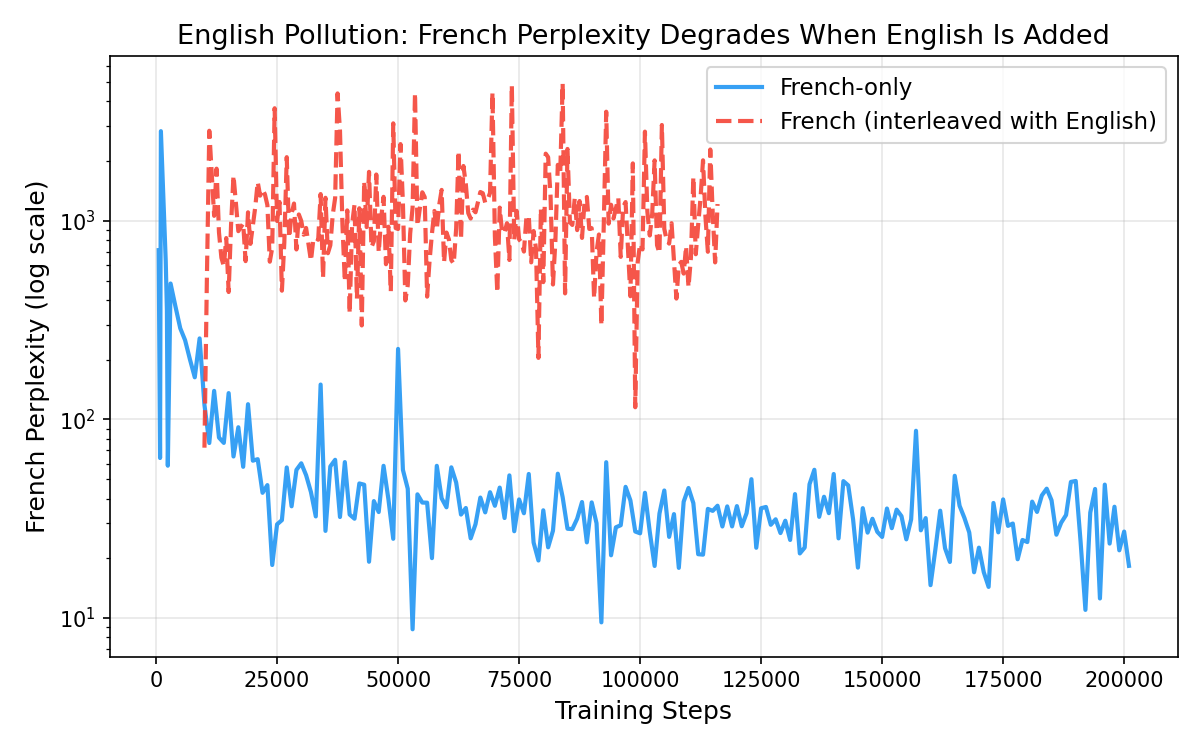
\includegraphics[width=0.65\textwidth]{figures/interleaved_ppx_only.png}
\captionof{figure}{Perplexity during interleaved French+English training. Blue (solid): French perplexity, which degrades catastrophically. Red (dotted): English perplexity, which is unaffected. The damage is asymmetric: English corrupts French, not the reverse.}
\end{minipage}
\vspace{1em}

\section{Introduction}

The title of this paper deliberately echoes Dijkstra's famous ``Go To Statement Considered Harmful'' (1968). Where Dijkstra argued that a ubiquitous programming practice was actively detrimental to software quality, we argue that a ubiquitous training practice---English-dominated corpora---may be actively detrimental to language model learning efficiency.

Modern English is morphologically impoverished. Through centuries of grammatical simplification \cite{mcwhorter2001power, dryer2013wals}, it has lost:
\begin{itemize}
    \item Grammatical gender and associated agreement
    \item Most case marking (from Old English's four cases to vestigial forms)
    \item Rich verb conjugation (minimal person/number agreement)
    \item Adjective-noun agreement
\end{itemize}

This poverty has a consequence that the field has overlooked: \textbf{English text provides sparse structural signal}. Where French marks gender and number redundantly across articles, adjectives, verbs, and participles---providing multiple views of the same grammatical relationship---English leaves these relationships implicit, recoverable only through word order and context.

We hypothesized that this difference would affect learning efficiency. We found something stronger: English does not merely fail to help; it actively \emph{hurts} when mixed with structurally explicit languages.

\subsection{Contributions}

\begin{enumerate}
    \item \textbf{Controlled cross-linguistic comparison}: First controlled experiment comparing training dynamics between fusional languages with different agreement richness (French vs.\ English), finding $\sim$50x efficiency advantage for French on grammatical acquisition.
    \item \textbf{Direct pollution evidence}: Interleaved French+English training degrades French grammar from 100\% to 50--70\%, demonstrating that English does not merely provide less signal; it actively corrupts structurally rich patterns when mixed in training.
    \item \textbf{Cross-domain replication}: The same interference pattern occurs when English is mixed with Rust code, establishing that the effect generalizes beyond natural language to any structurally explicit system.
    \item \textbf{Pollution hypothesis}: A theoretical framework explaining why English's implicit structure creates anti-signal that interferes with learning explicit structural patterns.
    \item \textbf{Orthogonality of metrics}: Discovery that perplexity and structural accuracy are orthogonal dimensions governed by different determinants (distributional coherence vs.\ morphological explicitness).
\end{enumerate}

\section{Related Work}

\subsection{Morphological Complexity in Language Modeling}

Prior work has examined how morphological properties affect language model performance, but has consistently conflated two orthogonal dimensions:

\textbf{Morphological complexity} (agglutinative languages like Turkish, Finnish): Many affixes, complex word formation, high type/token ratio. \cite{park2021morphology} found these languages harder to model with BPE tokenization.

\textbf{Agreement redundancy} (fusional languages with rich agreement like French, Russian): The same grammatical features are marked on multiple agreeing words. This dimension has been largely unexplored.

\cite{arnett2024morphology} compared agglutinative vs.\ fusional languages but did not compare fusional languages with different agreement richness. No prior work has compared French vs.\ English training dynamics under controlled conditions.

\subsection{Multilingual Training}

Multilingual models (mBERT, XLM-R, BLOOM) train on many languages simultaneously, but do not isolate the contribution of individual languages or examine interference effects. Our work suggests that English's presence in these corpora may be actively harming performance on other languages.

\subsection{Code Language Models}

Models like Codex, StarCoder, and CodeLlama are typically trained on code mixed with natural language. Our Rust experiment suggests this mixing may impair learning of structural patterns in the code itself.

\section{Experiment 1: French vs.\ English}

\subsection{Design}

We trained identical 125M parameter transformers on:
\begin{itemize}
    \item \textbf{English}: C4 corpus, English subset
    \item \textbf{French}: C4 corpus, French subset
\end{itemize}

All variables held constant: architecture (GPT-2 style, 12 layers, 768 hidden, 12 heads), hyperparameters (lr=6e-4, batch=2, seq=512), random seed (42), and tokenizer (joint 50K BPE trained on combined corpus).

Pre-registered on OSF (10.17605/OSF.IO/SJ48B) prior to data collection.

\subsection{Results}

\begin{table}[h]
\centering
\begin{tabular}{lccc}
\toprule
Metric & English & French & Ratio \\
\midrule
Perplexity (step 181k) & $\sim$1340 & $\sim$27 & $\sim$50x \\
Grammar probe accuracy & 40\% (chance) & 100\% & --- \\
Tokens to grammar saturation & $>$3B (not achieved) & $\sim$197M & $>$15x \\
\bottomrule
\end{tabular}
\caption{French vs.\ English training dynamics at 125M parameters.}
\end{table}

French achieved 100\% grammar probe accuracy by step 12,000 ($\sim$197M tokens) and maintained perfect accuracy with zero fluctuation thereafter. English fluctuated between 30--50\% (chance) throughout 3B tokens of training.

\subsection{Interpretation}

The 50x perplexity ratio and categorical difference in grammar acquisition cannot be explained by dataset artifacts. Both corpora come from C4 with identical preprocessing. The difference is the language itself.

French's agreement redundancy provides dense structural signal:

\textbf{French}: ``Les grandes portes sont ouvertes.'' Five words independently confirm gender and number.

\textbf{English}: ``The big doors are open.'' No explicit gender or number marking on most words.

\section{Experiment 2: Interleaved French+English}

\subsection{Motivation}

Experiment 1 established that French learns grammar 15x faster than English. But this alone does not prove pollution. Perhaps English simply provides less signal. To demonstrate active interference, we need to show that adding English to French \emph{degrades} French performance.

\subsection{Design}

We trained a single 125M transformer on interleaved French and English chunks (FR$_0$, EN$_0$, FR$_1$, EN$_1$, \ldots) for 200K steps, using the same architecture, hyperparameters, and data sources as Experiment 1.

\subsection{Results}

\begin{table}[h]
\centering
\begin{tabular}{lcc}
\toprule
Step & EN Grammar & FR Grammar \\
\midrule
12K & 40--50\% & 60--70\% \\
50K & 40\% & 60--70\% \\
74K & 40\% & 50--60\% \\
200K & 40\% & 50--60\% \\
\bottomrule
\end{tabular}
\caption{Interleaved training: French grammar degrades from 100\% (standalone) to 50--60\%.}
\end{table}

\textbf{Critical finding}: French grammar accuracy degraded from 100\% (French-only) to 50--70\% (interleaved), a catastrophic loss of grammatical competence caused solely by the presence of English in training.

\subsection{Interpretation}

This is the smoking gun for the pollution hypothesis:

\begin{enumerate}
    \item \textbf{English does not transfer}: English grammar never exceeded chance (40\%), despite exposure to French morphological patterns.
    \item \textbf{English actively corrupts}: French grammar dropped from 100\% to 50--60\%, far below standalone French performance at comparable token exposure.
    \item \textbf{The damage is asymmetric}: English remained unchanged while French was destroyed. This rules out simple ``dilution.'' If English merely provided less signal, French would still learn (just slower). Instead, English creates interference that specifically targets explicit structural patterns.
\end{enumerate}

\begin{figure}[h]
\centering
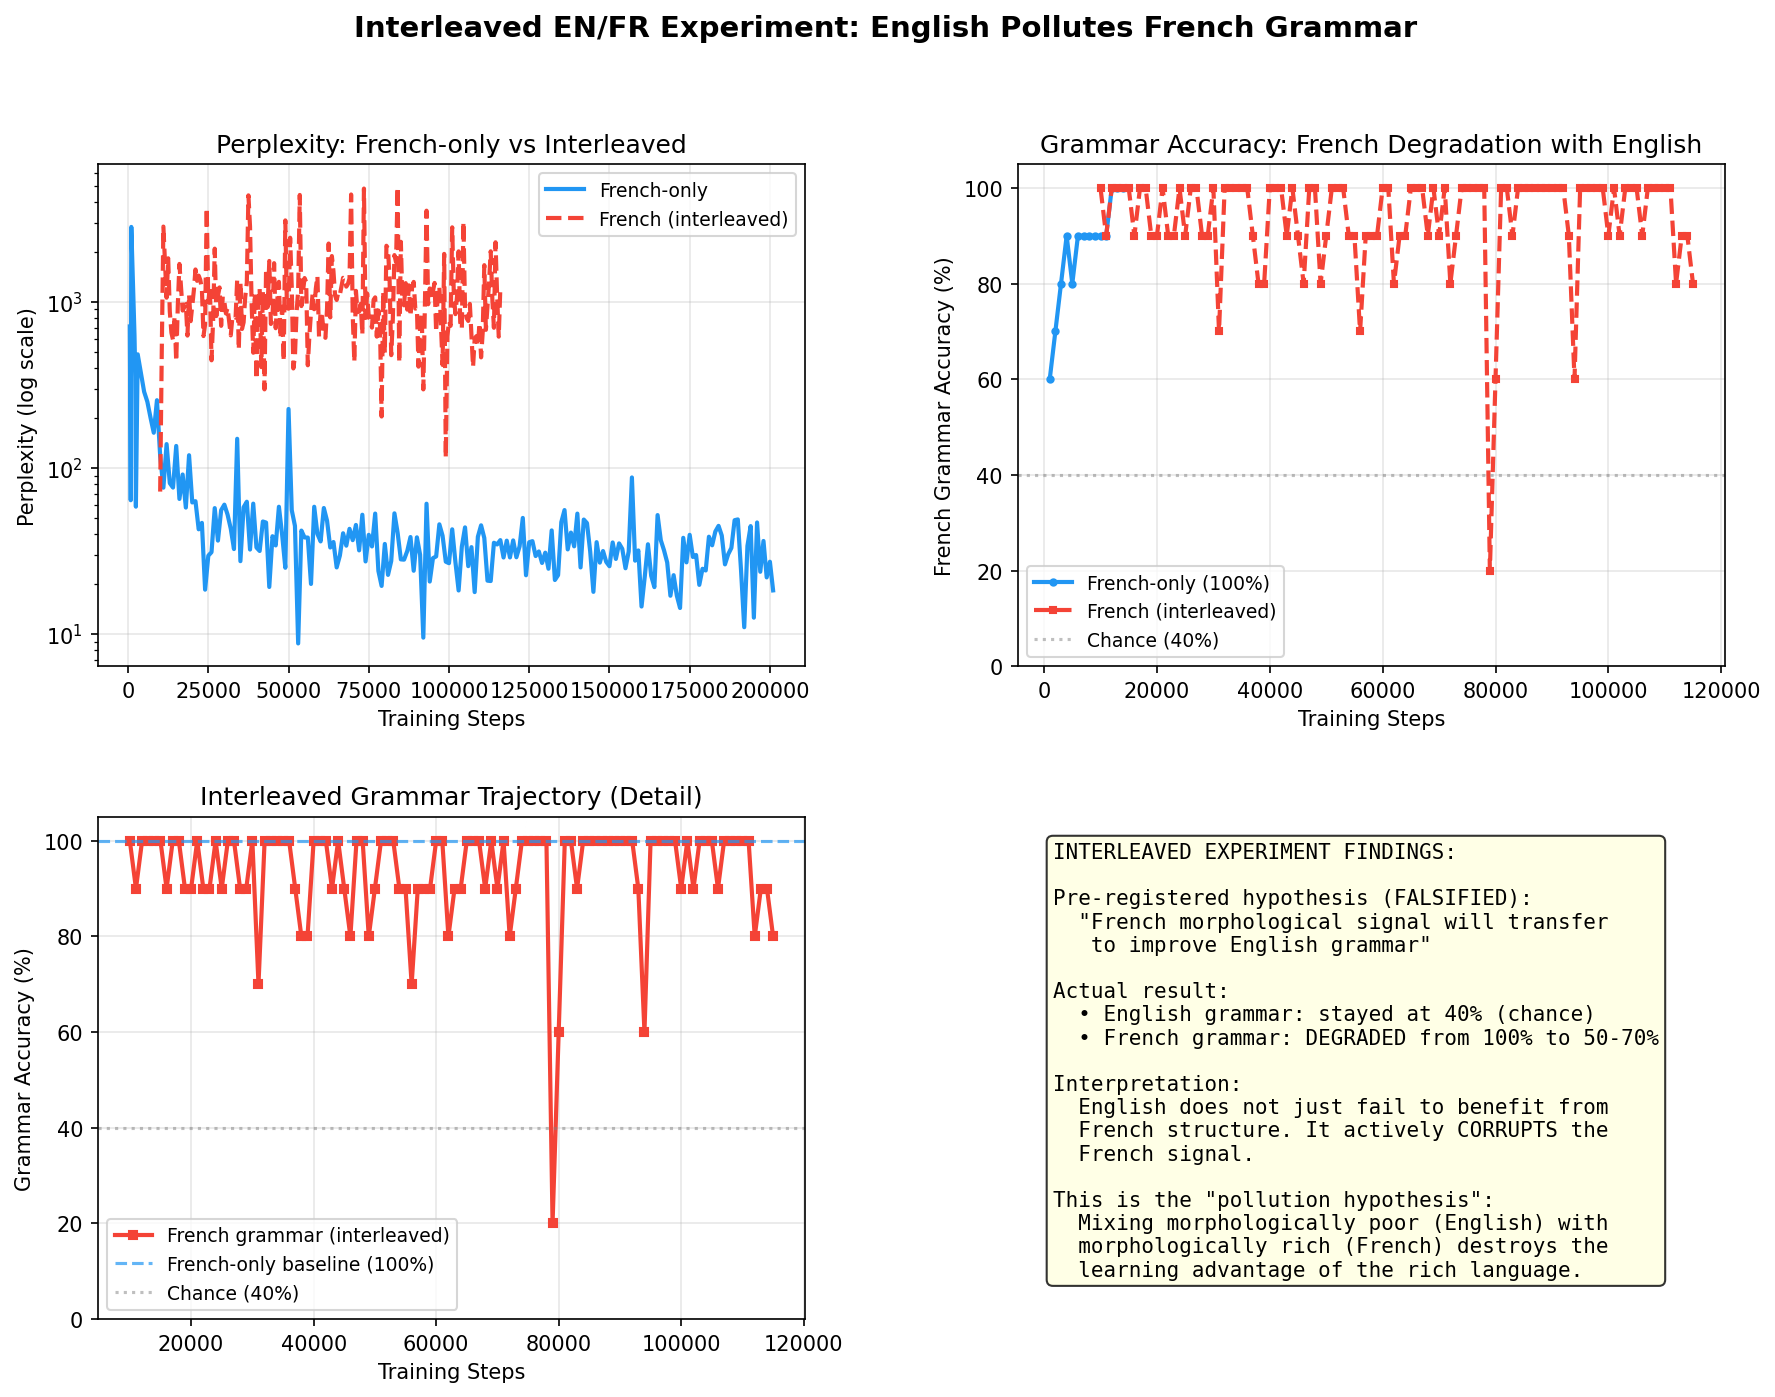
\includegraphics[width=0.9\textwidth]{figures/interleaved_experiment.png}
\caption{The interleaved EN/FR experiment showing English ``pollution'' of French grammar. Mixing English with French degrades French grammar from 100\% to 50--70\%.}
\end{figure}

\section{Experiment 3: Rust vs.\ Rust+English}

\subsection{Motivation}

If English's morphological poverty merely provides \emph{less} signal, mixing it with a rich language should dilute but not dramatically harm learning. But if English creates \emph{noise} that interferes with structural pattern recognition, we would expect active degradation.

Rust provides an ideal test case: its type system includes explicit structural markers analogous to natural language morphology: lifetime annotations, ownership markers, and the borrow checker.

\subsection{Results}

\begin{table}[h]
\centering
\begin{tabular}{lccc}
\toprule
Metric & Rust-only & Rust+English & Gap \\
\midrule
Perplexity & 49.7 & 510.5 & 10.27x \\
Probe accuracy & 86.7\% & 66.7\% & +20\% \\
\bottomrule
\end{tabular}
\caption{Rust vs.\ Rust+English at step 7,000.}
\end{table}

\begin{table}[h]
\centering
\begin{tabular}{lcc}
\toprule
Category & Rust-only & Rust+English \\
\midrule
Lifetime agreement & 100\% & 100\% \\
Ownership patterns & 67\% & 67\% \\
Type consistency & 100\% & 100\% \\
Borrow checker & \textbf{100\%} & 50\% \\
Mutability & \textbf{50\%} & 0\% \\
Expression syntax & \textbf{100\%} & 50\% \\
\bottomrule
\end{tabular}
\caption{Per-category probe accuracy at step 7,000.}
\end{table}

The PPX ratio \emph{accelerated} over training, widening from 4.84x to 11.36x. English is not merely diluting signal. It creates interference that compounds over time.

\subsection{Perplexity vs.\ Probe Accuracy: A Critical Distinction}

At step 9,500, an apparent paradox emerged: probe accuracy converged while the perplexity gap continued widening. This divergence reveals that perplexity and accuracy are orthogonal dimensions:

\begin{itemize}
    \item \textbf{Perplexity} = ``How narrow is my prediction distribution?'' (entropy)
    \item \textbf{Accuracy} = ``Have I learned the structural rules?'' (grammar)
\end{itemize}

These are independent dimensions. A model can have low perplexity without grammar (memorizing frequent patterns), or learn grammar while retaining high vocabulary entropy.

\textbf{Methodological implication}: Standard metrics (loss, perplexity) miss structural deficits. English models can improve perplexity indefinitely while never acquiring grammar.

\begin{figure}[h]
\centering
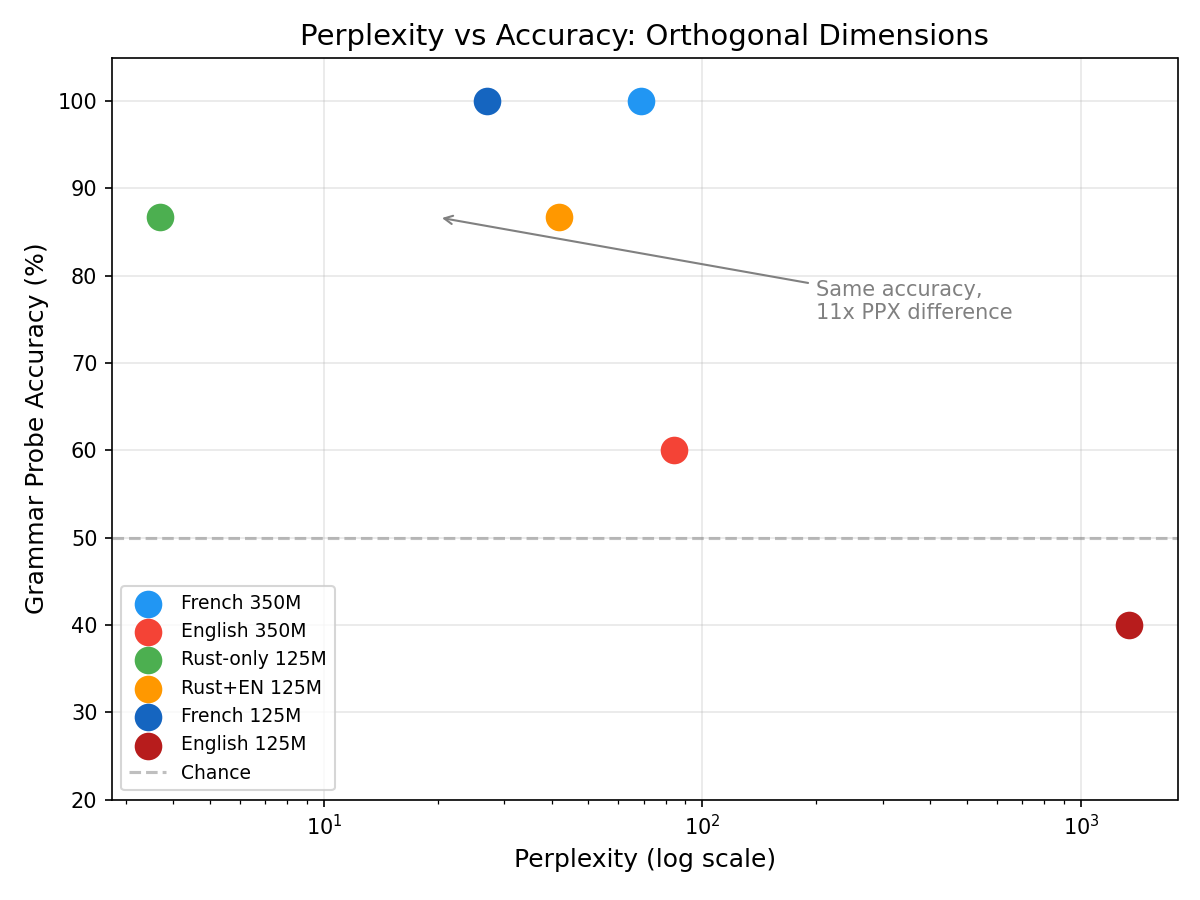
\includegraphics[width=0.9\textwidth]{figures/orthogonality.png}
\caption{PPX vs Accuracy scatter demonstrating orthogonality. Models can achieve identical probe accuracy with 13x different perplexity.}
\end{figure}

\section{The Pollution Hypothesis}

We propose that English text creates \textbf{structural noise} that interferes with pattern recognition:

\begin{enumerate}
    \item \textbf{Implicit structure is anti-signal}: English marks structure implicitly through word order. A model trained on English learns that structural information is \emph{not} explicitly marked. This creates a prior against looking for explicit markers.
    \item \textbf{Interference grows over time}: The widening PPX ratio suggests compound interference.
    \item \textbf{Category-specific effects}: Categories with explicit markers unique to Rust (borrow checker, mutability) showed the largest degradation. Categories shared with English-like syntax showed no degradation.
\end{enumerate}

\subsection{Implications for Multilingual Training}

If English pollutes learning of structured languages, the field's English-dominated corpora may be harming performance on morphologically rich languages, slowing acquisition of grammatical competence, and requiring more parameters to overcome interference.

\subsection{Implications for Code Models}

Training code models on code+English (comments, documentation) may impair learning of programming language structure. Pure-code training might achieve better structural competence with less compute.

\subsection{Scale Effects: A Conditional Factor}

\begin{table}[h]
\centering
\begin{tabular}{lcc}
\toprule
Condition & Emergence Step & Emergence Tokens \\
\midrule
French 125M & $\sim$4,000 & $\sim$4.1M \\
French 350M & $\sim$119,000 & $\sim$60.9M \\
English 125M & Not achieved & $>$14.3M \\
English 350M & Not achieved & $>$102.4M \\
\bottomrule
\end{tabular}
\caption{Scale is a conditional factor: larger models require more tokens for emergence in morphologically rich languages.}
\end{table}

For morphologically rich languages, larger models require 14.9x more tokens to achieve grammatical emergence. For morphologically poor languages, neither scale achieved grammar. The field's focus on scale as the path to capability may be an artifact of English-dominated training.

\begin{figure}[h]
\centering
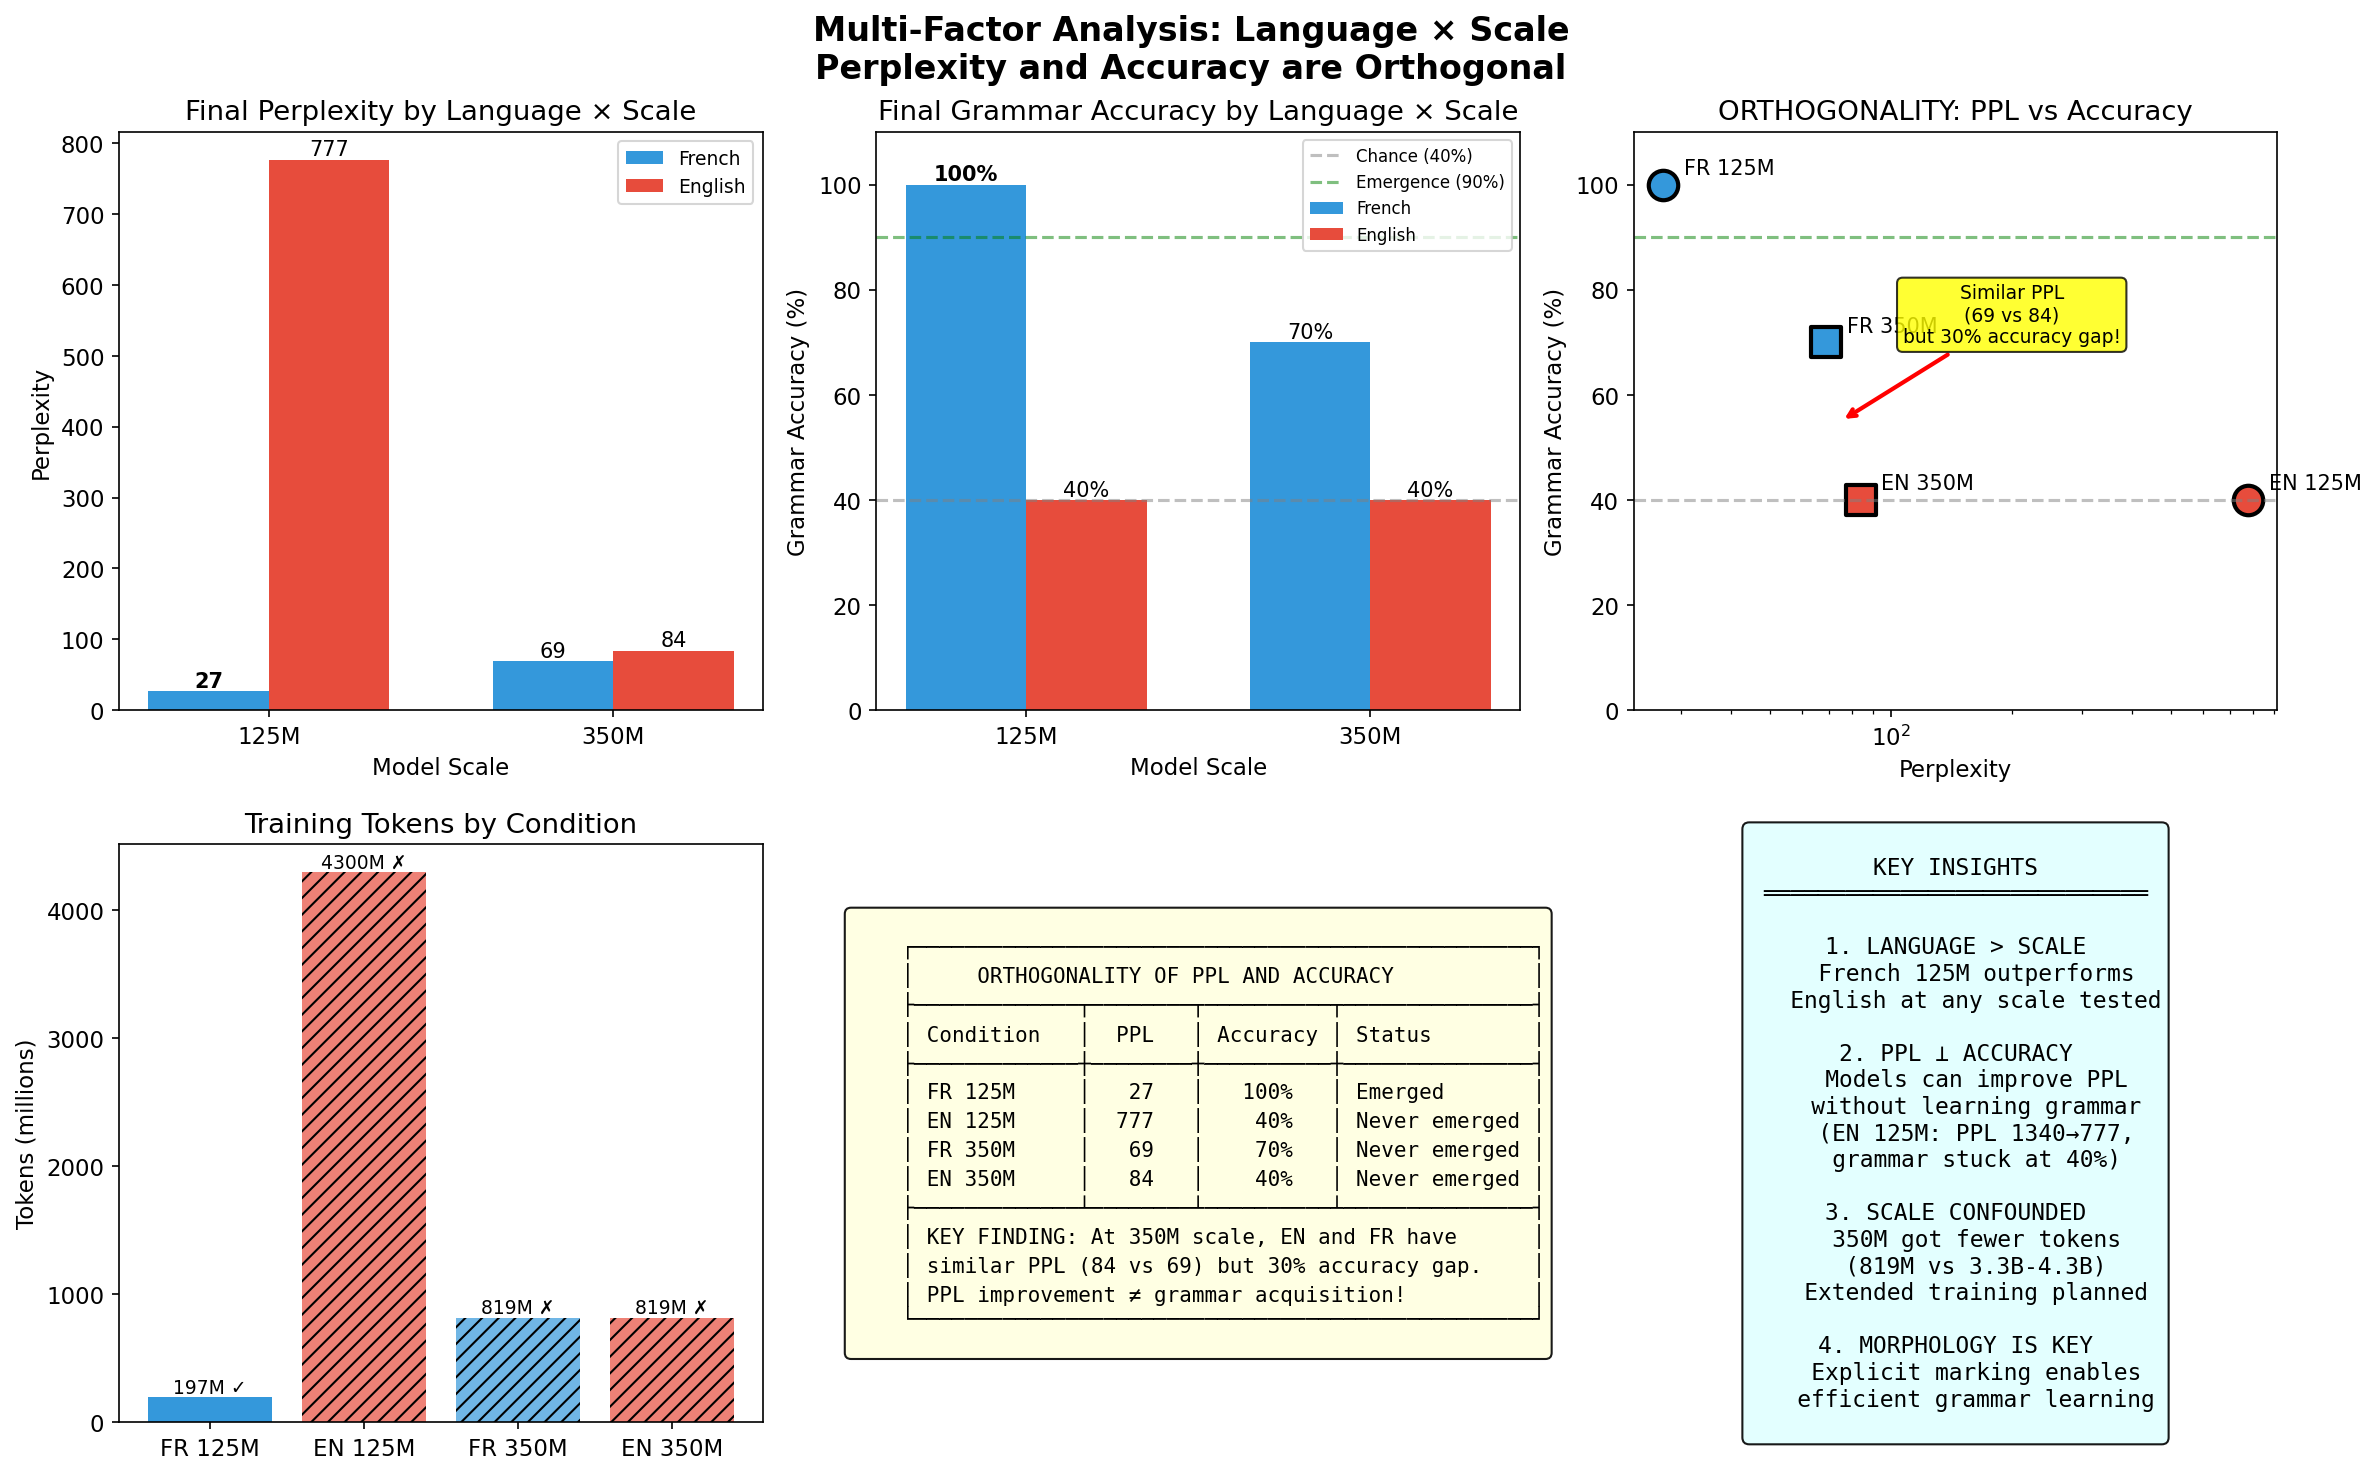
\includegraphics[width=0.9\textwidth]{figures/multifactor_analysis.png}
\caption{Multi-factor analysis (Language $\times$ Scale).}
\end{figure}

\section{Discussion}

\subsection{Why English Dominates}

English dominates LLM training for practical reasons: abundant digital text, economic importance, researcher demographics. Our results suggest this dominance has hidden costs.

\subsection{Remediation Strategies}

Possible approaches to reduce English pollution:
\begin{enumerate}
    \item \textbf{Staged training}: Train on structured languages first, then add English
    \item \textbf{Weighted sampling}: Reduce English proportion in multilingual corpora
    \item \textbf{Architecture modifications}: Separate pathways for implicit vs.\ explicit structure
\end{enumerate}

\subsection{Limitations}

Experiments conducted at 125M and 350M scale; larger models may show different dynamics. Limited probe sets. Rust is one programming language. Only two natural languages tested (French, English); other morphologically rich languages may show different patterns.

\section{Conclusion}

English is not a neutral training language. Its morphological poverty creates noise that actively interferes with learning structurally explicit patterns, whether in natural language (French) or code (Rust). The field's reliance on English-dominated corpora may be a hidden bottleneck.

We do not suggest abandoning English. It remains practically essential. But we suggest the field reconsider the assumption that more English is always better. In the context of structural pattern acquisition, English may be considered harmful.

\bibliographystyle{plainnat}
\begin{thebibliography}{9}

\bibitem[Arnett and Bergen(2024)]{arnett2024morphology}
C.~Arnett and B.~Bergen.
\newblock Why do language models perform worse for morphologically complex languages?
\newblock \emph{arXiv preprint}, 2024.

\bibitem[Dijkstra(1968)]{dijkstra1968goto}
E.~W. Dijkstra.
\newblock Go to statement considered harmful.
\newblock \emph{Communications of the ACM}, 11(3):147--148, 1968.

\bibitem[Park et~al.(2021)]{park2021morphology}
J.~Park et~al.
\newblock Morphology matters: A multilingual language modeling analysis.
\newblock \emph{TACL}, 9:261--276, 2021.

\bibitem[Sennrich and Haddow(2016)]{sennrich2016linguistic}
R.~Sennrich and B.~Haddow.
\newblock Linguistic input features improve neural machine translation.
\newblock In \emph{WMT}, 2016.

\bibitem[McWhorter(2001)]{mcwhorter2001power}
J.~McWhorter.
\newblock \emph{The Power of Babel: A Natural History of Language}.
\newblock Times Books, 2001.

\bibitem[Dryer and Haspelmath(2013)]{dryer2013wals}
M.~S. Dryer and M.~Haspelmath, editors.
\newblock \emph{WALS Online (v2020)}.
\newblock Zenodo, 2013.
\newblock \url{https://doi.org/10.5281/zenodo.7385533}

\bibitem[Wasserman(2026)]{wasserman2026scaling}
A.~Z. Wasserman.
\newblock The scaling hypothesis is language-contingent: Evidence from cross-linguistic training dynamics.
\newblock \emph{Zenodo preprint}, 2026.
\newblock \url{https://doi.org/10.5281/ZENODO.19423151}

\end{thebibliography}

\appendix
\section{Pre-registration}

OSF 10.17605/OSF.IO/SJ48B. Pre-registered prior to data collection.

Code and training logs: \url{https://github.com/adamzwasserman/fractal-language}

\end{document}
